% Generated by Sphinx.
\def\sphinxdocclass{report}
\documentclass[letterpaper,10pt,dvipdfmx,openany]{sphinxmanual}
\usepackage[utf8]{inputenc}
\DeclareUnicodeCharacter{00A0}{\nobreakspace}
\usepackage{cmap}
\usepackage[T1]{fontenc}

\usepackage{times}

\usepackage{longtable}
\usepackage{sphinx}
\usepackage{multirow}
\usepackage{pxjahyper}

\title{Shiftk Documentation}
\date{2017 年 01 月 27 日}
\release{0.1}
\author{kawamura}
\newcommand{\sphinxlogo}{}
\renewcommand{\releasename}{リリース}
\makeindex

\makeatletter
\def\PYG@reset{\let\PYG@it=\relax \let\PYG@bf=\relax%
    \let\PYG@ul=\relax \let\PYG@tc=\relax%
    \let\PYG@bc=\relax \let\PYG@ff=\relax}
\def\PYG@tok#1{\csname PYG@tok@#1\endcsname}
\def\PYG@toks#1+{\ifx\relax#1\empty\else%
    \PYG@tok{#1}\expandafter\PYG@toks\fi}
\def\PYG@do#1{\PYG@bc{\PYG@tc{\PYG@ul{%
    \PYG@it{\PYG@bf{\PYG@ff{#1}}}}}}}
\def\PYG#1#2{\PYG@reset\PYG@toks#1+\relax+\PYG@do{#2}}

\expandafter\def\csname PYG@tok@gd\endcsname{\def\PYG@tc##1{\textcolor[rgb]{0.63,0.00,0.00}{##1}}}
\expandafter\def\csname PYG@tok@gu\endcsname{\let\PYG@bf=\textbf\def\PYG@tc##1{\textcolor[rgb]{0.50,0.00,0.50}{##1}}}
\expandafter\def\csname PYG@tok@gt\endcsname{\def\PYG@tc##1{\textcolor[rgb]{0.00,0.27,0.87}{##1}}}
\expandafter\def\csname PYG@tok@gs\endcsname{\let\PYG@bf=\textbf}
\expandafter\def\csname PYG@tok@gr\endcsname{\def\PYG@tc##1{\textcolor[rgb]{1.00,0.00,0.00}{##1}}}
\expandafter\def\csname PYG@tok@cm\endcsname{\let\PYG@it=\textit\def\PYG@tc##1{\textcolor[rgb]{0.25,0.50,0.56}{##1}}}
\expandafter\def\csname PYG@tok@vg\endcsname{\def\PYG@tc##1{\textcolor[rgb]{0.73,0.38,0.84}{##1}}}
\expandafter\def\csname PYG@tok@m\endcsname{\def\PYG@tc##1{\textcolor[rgb]{0.13,0.50,0.31}{##1}}}
\expandafter\def\csname PYG@tok@mh\endcsname{\def\PYG@tc##1{\textcolor[rgb]{0.13,0.50,0.31}{##1}}}
\expandafter\def\csname PYG@tok@cs\endcsname{\def\PYG@tc##1{\textcolor[rgb]{0.25,0.50,0.56}{##1}}\def\PYG@bc##1{\setlength{\fboxsep}{0pt}\colorbox[rgb]{1.00,0.94,0.94}{\strut ##1}}}
\expandafter\def\csname PYG@tok@ge\endcsname{\let\PYG@it=\textit}
\expandafter\def\csname PYG@tok@vc\endcsname{\def\PYG@tc##1{\textcolor[rgb]{0.73,0.38,0.84}{##1}}}
\expandafter\def\csname PYG@tok@il\endcsname{\def\PYG@tc##1{\textcolor[rgb]{0.13,0.50,0.31}{##1}}}
\expandafter\def\csname PYG@tok@go\endcsname{\def\PYG@tc##1{\textcolor[rgb]{0.20,0.20,0.20}{##1}}}
\expandafter\def\csname PYG@tok@cp\endcsname{\def\PYG@tc##1{\textcolor[rgb]{0.00,0.44,0.13}{##1}}}
\expandafter\def\csname PYG@tok@gi\endcsname{\def\PYG@tc##1{\textcolor[rgb]{0.00,0.63,0.00}{##1}}}
\expandafter\def\csname PYG@tok@gh\endcsname{\let\PYG@bf=\textbf\def\PYG@tc##1{\textcolor[rgb]{0.00,0.00,0.50}{##1}}}
\expandafter\def\csname PYG@tok@ni\endcsname{\let\PYG@bf=\textbf\def\PYG@tc##1{\textcolor[rgb]{0.84,0.33,0.22}{##1}}}
\expandafter\def\csname PYG@tok@nl\endcsname{\let\PYG@bf=\textbf\def\PYG@tc##1{\textcolor[rgb]{0.00,0.13,0.44}{##1}}}
\expandafter\def\csname PYG@tok@nn\endcsname{\let\PYG@bf=\textbf\def\PYG@tc##1{\textcolor[rgb]{0.05,0.52,0.71}{##1}}}
\expandafter\def\csname PYG@tok@no\endcsname{\def\PYG@tc##1{\textcolor[rgb]{0.38,0.68,0.84}{##1}}}
\expandafter\def\csname PYG@tok@na\endcsname{\def\PYG@tc##1{\textcolor[rgb]{0.25,0.44,0.63}{##1}}}
\expandafter\def\csname PYG@tok@nb\endcsname{\def\PYG@tc##1{\textcolor[rgb]{0.00,0.44,0.13}{##1}}}
\expandafter\def\csname PYG@tok@nc\endcsname{\let\PYG@bf=\textbf\def\PYG@tc##1{\textcolor[rgb]{0.05,0.52,0.71}{##1}}}
\expandafter\def\csname PYG@tok@nd\endcsname{\let\PYG@bf=\textbf\def\PYG@tc##1{\textcolor[rgb]{0.33,0.33,0.33}{##1}}}
\expandafter\def\csname PYG@tok@ne\endcsname{\def\PYG@tc##1{\textcolor[rgb]{0.00,0.44,0.13}{##1}}}
\expandafter\def\csname PYG@tok@nf\endcsname{\def\PYG@tc##1{\textcolor[rgb]{0.02,0.16,0.49}{##1}}}
\expandafter\def\csname PYG@tok@si\endcsname{\let\PYG@it=\textit\def\PYG@tc##1{\textcolor[rgb]{0.44,0.63,0.82}{##1}}}
\expandafter\def\csname PYG@tok@s2\endcsname{\def\PYG@tc##1{\textcolor[rgb]{0.25,0.44,0.63}{##1}}}
\expandafter\def\csname PYG@tok@vi\endcsname{\def\PYG@tc##1{\textcolor[rgb]{0.73,0.38,0.84}{##1}}}
\expandafter\def\csname PYG@tok@nt\endcsname{\let\PYG@bf=\textbf\def\PYG@tc##1{\textcolor[rgb]{0.02,0.16,0.45}{##1}}}
\expandafter\def\csname PYG@tok@nv\endcsname{\def\PYG@tc##1{\textcolor[rgb]{0.73,0.38,0.84}{##1}}}
\expandafter\def\csname PYG@tok@s1\endcsname{\def\PYG@tc##1{\textcolor[rgb]{0.25,0.44,0.63}{##1}}}
\expandafter\def\csname PYG@tok@gp\endcsname{\let\PYG@bf=\textbf\def\PYG@tc##1{\textcolor[rgb]{0.78,0.36,0.04}{##1}}}
\expandafter\def\csname PYG@tok@sh\endcsname{\def\PYG@tc##1{\textcolor[rgb]{0.25,0.44,0.63}{##1}}}
\expandafter\def\csname PYG@tok@ow\endcsname{\let\PYG@bf=\textbf\def\PYG@tc##1{\textcolor[rgb]{0.00,0.44,0.13}{##1}}}
\expandafter\def\csname PYG@tok@sx\endcsname{\def\PYG@tc##1{\textcolor[rgb]{0.78,0.36,0.04}{##1}}}
\expandafter\def\csname PYG@tok@bp\endcsname{\def\PYG@tc##1{\textcolor[rgb]{0.00,0.44,0.13}{##1}}}
\expandafter\def\csname PYG@tok@c1\endcsname{\let\PYG@it=\textit\def\PYG@tc##1{\textcolor[rgb]{0.25,0.50,0.56}{##1}}}
\expandafter\def\csname PYG@tok@kc\endcsname{\let\PYG@bf=\textbf\def\PYG@tc##1{\textcolor[rgb]{0.00,0.44,0.13}{##1}}}
\expandafter\def\csname PYG@tok@c\endcsname{\let\PYG@it=\textit\def\PYG@tc##1{\textcolor[rgb]{0.25,0.50,0.56}{##1}}}
\expandafter\def\csname PYG@tok@mf\endcsname{\def\PYG@tc##1{\textcolor[rgb]{0.13,0.50,0.31}{##1}}}
\expandafter\def\csname PYG@tok@err\endcsname{\def\PYG@bc##1{\setlength{\fboxsep}{0pt}\fcolorbox[rgb]{1.00,0.00,0.00}{1,1,1}{\strut ##1}}}
\expandafter\def\csname PYG@tok@kd\endcsname{\let\PYG@bf=\textbf\def\PYG@tc##1{\textcolor[rgb]{0.00,0.44,0.13}{##1}}}
\expandafter\def\csname PYG@tok@ss\endcsname{\def\PYG@tc##1{\textcolor[rgb]{0.32,0.47,0.09}{##1}}}
\expandafter\def\csname PYG@tok@sr\endcsname{\def\PYG@tc##1{\textcolor[rgb]{0.14,0.33,0.53}{##1}}}
\expandafter\def\csname PYG@tok@mo\endcsname{\def\PYG@tc##1{\textcolor[rgb]{0.13,0.50,0.31}{##1}}}
\expandafter\def\csname PYG@tok@mi\endcsname{\def\PYG@tc##1{\textcolor[rgb]{0.13,0.50,0.31}{##1}}}
\expandafter\def\csname PYG@tok@kn\endcsname{\let\PYG@bf=\textbf\def\PYG@tc##1{\textcolor[rgb]{0.00,0.44,0.13}{##1}}}
\expandafter\def\csname PYG@tok@o\endcsname{\def\PYG@tc##1{\textcolor[rgb]{0.40,0.40,0.40}{##1}}}
\expandafter\def\csname PYG@tok@kr\endcsname{\let\PYG@bf=\textbf\def\PYG@tc##1{\textcolor[rgb]{0.00,0.44,0.13}{##1}}}
\expandafter\def\csname PYG@tok@s\endcsname{\def\PYG@tc##1{\textcolor[rgb]{0.25,0.44,0.63}{##1}}}
\expandafter\def\csname PYG@tok@kp\endcsname{\def\PYG@tc##1{\textcolor[rgb]{0.00,0.44,0.13}{##1}}}
\expandafter\def\csname PYG@tok@w\endcsname{\def\PYG@tc##1{\textcolor[rgb]{0.73,0.73,0.73}{##1}}}
\expandafter\def\csname PYG@tok@kt\endcsname{\def\PYG@tc##1{\textcolor[rgb]{0.56,0.13,0.00}{##1}}}
\expandafter\def\csname PYG@tok@sc\endcsname{\def\PYG@tc##1{\textcolor[rgb]{0.25,0.44,0.63}{##1}}}
\expandafter\def\csname PYG@tok@sb\endcsname{\def\PYG@tc##1{\textcolor[rgb]{0.25,0.44,0.63}{##1}}}
\expandafter\def\csname PYG@tok@k\endcsname{\let\PYG@bf=\textbf\def\PYG@tc##1{\textcolor[rgb]{0.00,0.44,0.13}{##1}}}
\expandafter\def\csname PYG@tok@se\endcsname{\let\PYG@bf=\textbf\def\PYG@tc##1{\textcolor[rgb]{0.25,0.44,0.63}{##1}}}
\expandafter\def\csname PYG@tok@sd\endcsname{\let\PYG@it=\textit\def\PYG@tc##1{\textcolor[rgb]{0.25,0.44,0.63}{##1}}}

\def\PYGZbs{\char`\\}
\def\PYGZus{\char`\_}
\def\PYGZob{\char`\{}
\def\PYGZcb{\char`\}}
\def\PYGZca{\char`\^}
\def\PYGZam{\char`\&}
\def\PYGZlt{\char`\<}
\def\PYGZgt{\char`\>}
\def\PYGZsh{\char`\#}
\def\PYGZpc{\char`\%}
\def\PYGZdl{\char`\$}
\def\PYGZhy{\char`\-}
\def\PYGZsq{\char`\'}
\def\PYGZdq{\char`\"}
\def\PYGZti{\char`\~}
% for compatibility with earlier versions
\def\PYGZat{@}
\def\PYGZlb{[}
\def\PYGZrb{]}
\makeatother

\begin{document}

\maketitle
\tableofcontents
\phantomsection\label{index::doc}



\chapter{概要}
\label{shiftk_overview_ja:welcome-to-sample-program-s-documentation}\label{shiftk_overview_ja::doc}\label{shiftk_overview_ja:id1}
本資料はISSP Math
Libraryの内の, Krylov部分空間法に基づくシフト線形方程式群ライブラリ
\(K(\omega)\) を用いた Green関数計算用ミニアプリのマニュアルです.
ライブラリに関する使用方法については, '' \(K(\omega)\) マニュアル''に記載しました.


\section{ソフトウェア概要}
\label{shiftk_overview_ja:id2}
本ソフトウェアでは, Green関数
\begin{gather}
\begin{split}\begin{align}
G_{i}(z) =
\langle i | (z-{\hat H})^{-1}| i \rangle
\equiv
{\boldsymbol \varphi}_i^{*} \cdot (z-{\hat H})^{-1} {\boldsymbol \varphi}_i
\end{align}\end{split}\notag
\end{gather}
の計算を行います.
ここで \(| i \rangle\) はベクトル, \({\cal H}\) はハミルトニアン,
\(z\) は複素数シフトを表します.

なお \({\cal H}\) については,
\begin{itemize}
\item {} 
\({\cal H}\) をMatrixMarket形式の入力ファイルとして与えるモード

\item {} 
Heisenberg模型の \({\cal H}\) を内部で与えるモード

\end{itemize}

を用意します.
またグリーン関数の計算では, \({\hat H}\) と \(z\) が複素数もしくは実数かに応じ,
\begin{itemize}
\item {} 
\({\hat H}\) も \(z\) も両方複素数の場合 : Shifted
Bi-Conjugate Gradient(BiCG)法

\item {} 
\({\hat H}\) が実数で \(z\) が複素数の場合 : Shifted
Conjugate Orthogonal Conjugate Gradient(COCG)法

\end{itemize}

の手法を用意しています.


\chapter{ライセンス}
\label{shiftk_copy_ja::doc}\label{shiftk_copy_ja:id1}
\emph{© 2016- The University of Tokyo. All rights reserved.}

\begin{DUlineblock}{0em}
\item[] This software is developed under the support of
\item[] ``\emph{Project for advancement of software usability in materials science}'' by The
\item[] Institute for Solid State Physics, The University of Tokyo.
\item[] 
\item[] This library is free software; you can redistribute it and/or
\item[] modify it under the terms of the GNU Lesser General Public
\item[] License as published by the Free Software Foundation; either
\item[] version 2.1 of the License, or (at your option) any later version.
\item[] This library is distributed in the hope that it will be useful,
\item[] but WITHOUT ANY WARRANTY; without even the implied warranty of
\item[] MERCHANTABILITY or FITNESS FOR A PARTICULAR PURPOSE. See the GNU
\item[] Lesser General Public License for more details.
\item[] 
\item[] You should have received a copy of the GNU Lesser General Public
\item[] License along with this library; if not, write to the Free Software
\item[] Foundation, Inc., 59 Temple Place, Suite 330, Boston, MA 02111-1307 USA
\item[] 
\item[] For more details, See ‘COPYING.LESSER’ in the root directory of this library.
\end{DUlineblock}


\chapter{要件}
\label{shiftk_env_ja::doc}\label{shiftk_env_ja:id1}\begin{itemize}
\item {} 
fortranコンパイラー

\item {} 
K \(omega\) ライブラリ

\item {} 
BLAS, LAPACK

\item {} 
MPIライブラリ(Oprional)

\end{itemize}


\chapter{計算の流れ}
\label{shiftk_flow_ja::doc}\label{shiftk_flow_ja:id1}
本ソフトウェアでは
\begin{enumerate}
\item {} 
条件ファイルの読み込み

\item {} 
(オプション)入力ファイルの読み込み (ハミルトニアン, ベクトルなど)

\item {} 
(オプション)リスタート用ファイルの読み込み (係数, 残差ベクトルなど)

\item {} 
ライブラリを利用したループ計算

\item {} 
計算結果ファイル出力(係数, 残差ベクトル, 動的グリーン関数)

\end{enumerate}

の流れで計算を行います
(図 \ref{shiftk_flow_ja:calcflow} ).
使用の流れおよび各ファイルの詳細については, {\hyperref[shiftk_flow_ja:usage]{\emph{使用の流れ}}} ,
{\hyperref[shiftk_format_ja:fileformat]{\emph{ファイルフォーマット}}} にそれぞれ記載してあります.
\begin{figure}[htbp]
\centering
\capstart

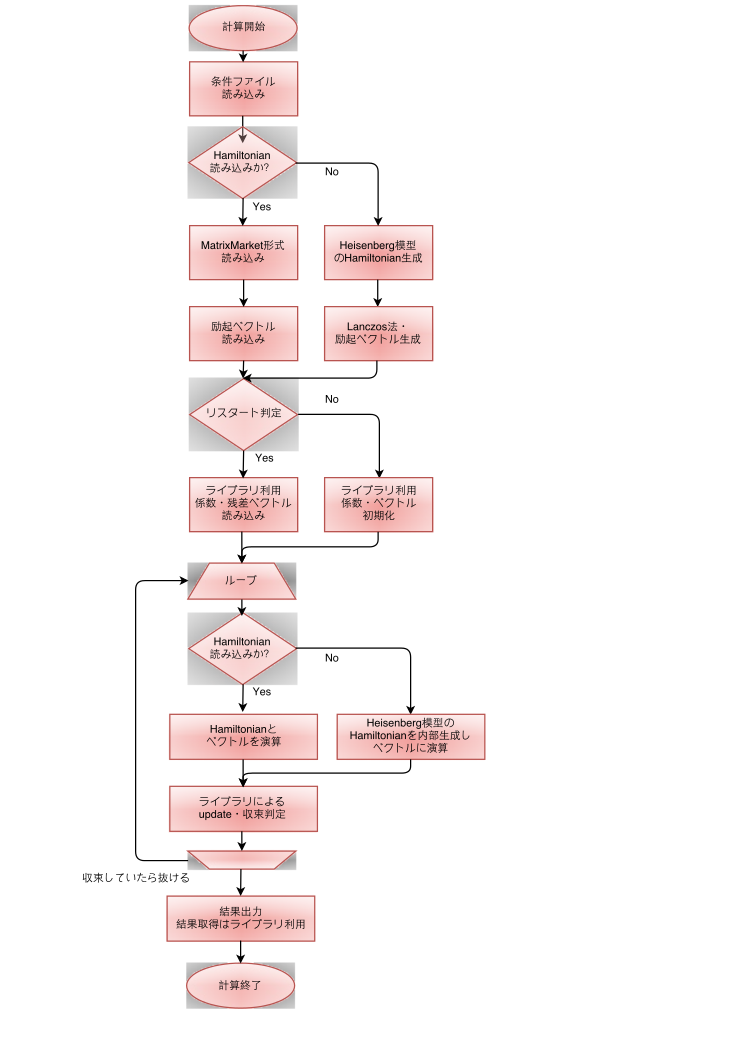
\includegraphics{flow.png}
\caption{計算の流れ.}\label{shiftk_flow_ja:calcflow}\end{figure}


\section{使用の流れ}
\label{shiftk_flow_ja:usage}\label{shiftk_flow_ja:id2}

\section{(リスタートではない)通常の計算}
\label{shiftk_flow_ja:id3}

\subsection{入力条件ファイルの作成}
\label{shiftk_flow_ja:id4}
周波数や計算時のループ回数の最大数などを指定するファイルを作成します.

以下に入力ファイルの例を示します.

\begin{Verbatim}[commandchars=\\\{\}]
\PYGZam{}filename
  inham = \PYGZdq{}\PYGZdq{}
  invec = \PYGZdq{}\PYGZdq{}
/
\PYGZam{}ham
nsite = 4
Jx = 1d0
Jy = 1d0
Jz = 1d0
Dz = 0d0
/
\PYGZam{}cg
  maxloops = 100
  convfactor = 6
/
\PYGZam{}dyn
  calctype = \PYGZdq{}normal\PYGZdq{}
  nomega = 100
  omegamin = (\PYGZhy{}2d0, 0.1d0)
  omegamax = ( 1d0, 0.1d0)
  outrestart = .TRUE.
/
\end{Verbatim}

ここで
\code{InHam} はMatrixMarket形式に従ったハミルトニアンの要素が記載されたファイル名,
\code{InVec} は励起ベクトルが記載されたファイル名です. また,
\code{OmegaMin} は \(z\) の始点,
\code{OmegaMax} は \(z\) の終点 に対応します.
``(実部,虚部)''の形式で入力してください.
\code{NOmega} は動的グリーン関数を求めるための周波数
\begin{gather}
\begin{split}\begin{align}
\omega_n =  {\tt OmegaMin}
+ \frac{n-1}{{\tt NOmega}-1}({\tt OmegaMax} - {\tt OmegaMin}),
\end{align}\end{split}\notag
\end{gather}
(\(n=1\cdots\) \code{NOmega})を指定するための変数です.
また,  \code{MaxLoops} はループの最大数を指定します.  残りの変数の説明や
省略可能な変数など, 入力条件ファイルの詳細はSec.
{\hyperref[shiftk_format_ja:modpara]{\emph{ファイル名および計算条件指定ファイル}}} を参照してください.
また文字列変数は \code{'} もしくは \code{"} で囲ってください.


\subsection{(オプション)入力ファイルの作成}
\label{shiftk_flow_ja:id5}
MatrixMarket形式に従ったハミルトニアンの要素が記載されたファイルと
励起ベクトルを記載したファイルを作成します.

以下に励起ベクトルのファイル例を示します.

\begin{Verbatim}[commandchars=\\\{\}]
256
0.01    0.0
0.05    0.0
0.1     0.0
(continue ...)
\end{Verbatim}

ファイル形式は {\hyperref[shiftk_format_ja:ham]{\emph{InHamファイル}}}, {\hyperref[shiftk_format_ja:vec]{\emph{InVecファイル}}} を参照してください.


\subsection{計算実行}
\label{shiftk_flow_ja:id6}
作成した入力ファイル指定ファイルを引数にして計算実行します.
計算の途中経過は標準出力されます. 以下, 実行ファイルを \code{ShiftK.out} ,
入力ファイル指定ファイルを \code{namelist.def} としてコマンド例を記載します.

\begin{Verbatim}[commandchars=\\\{\}]
\PYG{n+nv}{\PYGZdl{} }ShiftK.out namelist.def
\end{Verbatim}


\subsection{計算結果出力}
\label{shiftk_flow_ja:id7}
以下のファイルが \code{output} フォルダに出力されます.

\begin{Verbatim}[commandchars=\\\{\}]
\PYG{n}{TriDiagComp}\PYG{o}{.}\PYG{n}{dat}\PYG{p}{,} \PYG{n}{ResVec}\PYG{o}{.}\PYG{n}{dat}\PYG{p}{,} \PYG{n}{dynamicalG}\PYG{o}{.}\PYG{n}{dat}
\end{Verbatim}

ここで,
\code{TriDiagComp.dat} はリスタート用の係数およびノルムが格納されているファイル,
\code{ResVec.dat} はリスタート用の残差ベクトルが格納されているファイル,
\code{dynamicalG.dat} は動的グリーン関数の計算結果が格納されているファイルをそれぞれ表します.
各ファイルのフォーマットは
{\hyperref[shiftk_format_ja:revec]{\emph{リスタート用ベクトル}}} - {\hyperref[shiftk_format_ja:dynamicalg]{\emph{動的グリーン関数ファイル}}} を参照ください.


\section{動的グリーン関数の再計算を行う場合}
\label{shiftk_flow_ja:id8}
動的グリーン関数を求めた際に出力される \code{TriDiagComp.dat} および \code{ResVec.dat} を用い,
異なる周波数での動的グリーン関数を再計算する場合の流れを示します.


\subsection{入力条件ファイルの作成}
\label{shiftk_flow_ja:id9}
\code{namelist.def} 内の \code{calctype} パラメーターを \code{"normal"} から \code{"recalc"}
に変更のうえ,  \code{OmegaMin} 等その他のパラメーターをお好きなように変更してください.
\code{InHam} ,  \code{InVec} およびそれらのファイルの中身は変更しないでください.


\subsection{計算実行}
\label{shiftk_flow_ja:id10}
作成した入力ファイル指定ファイルを引数にして計算実行します.
\code{output/} フォルダにある \code{TriDiagComp.dat} および \code{ResVec.dat} が自動的に読み込まれます.
計算の途中経過は標準出力されます.
なお,  \code{output/} フォルダ内に \code{dynamicalG.dat} が存在する場合は計算終了時に上書きされます.

以下, 実行ファイルを \code{ShiftK.out} ,
入力ファイル指定ファイルを \code{namelist.def} としてコマンド例を記載します.

\begin{Verbatim}[commandchars=\\\{\}]
\PYG{n+nv}{\PYGZdl{} }ShiftK.out namelist.def
\end{Verbatim}


\subsection{計算結果出力}
\label{shiftk_flow_ja:id11}
\code{output/} フォルダ内にある \code{dynamicalG.dat} が
出力(同名のファイルが存在する場合には上書き)されます.


\section{リスタート計算をする場合}
\label{shiftk_flow_ja:id12}

\subsection{入力条件ファイルの作成}
\label{shiftk_flow_ja:id13}
\code{namelist.def} 内の \code{calctype} パラメーターを \code{"restart"} に変更してください.
あとは上記の再計算の場合と同様です.


\subsection{計算実行}
\label{shiftk_flow_ja:id14}
作成した入力ファイル指定ファイルを引数にして計算実行します.
計算の途中経過は標準出力されます.  以下, 実行ファイルを \code{ShiftK.out}
,
入力ファイル指定ファイルを \code{namelist.def} としてコマンド例を記載します.

\begin{Verbatim}[commandchars=\\\{\}]
\PYG{n+nv}{\PYGZdl{} }ShiftK.out namelist.def
\end{Verbatim}


\subsection{計算結果出力}
\label{shiftk_flow_ja:id15}
以下のファイルが \code{output/} フォルダに出力されます.

\begin{Verbatim}[commandchars=\\\{\}]
\PYG{n}{TriDiagComp}\PYG{o}{.}\PYG{n}{dat}\PYG{p}{,} \PYG{n}{ResVec}\PYG{o}{.}\PYG{n}{dat}\PYG{p}{,} \PYG{n}{dynamicalG}\PYG{o}{.}\PYG{n}{dat}
\end{Verbatim}

ここで,
\code{TriDiagComp.dat} はリスタート用の係数およびノルムが格納されているファイル,
\code{ResVec.dat} はリスタート用の残差ベクトルが格納されているファイル,
\code{dynamicalG.dat} は動的グリーン関数の計算結果が格納されているファイルをそれぞれ表します.
各ファイルのフォーマットは, {\hyperref[shiftk_format_ja:revec]{\emph{リスタート用ベクトル}}} - {\hyperref[shiftk_format_ja:dynamicalg]{\emph{動的グリーン関数ファイル}}} を参照ください.


\chapter{ファイルフォーマット}
\label{shiftk_format_ja::doc}\label{shiftk_format_ja:fileformat}\label{shiftk_format_ja:id1}

\section{入力ファイル}
\label{shiftk_format_ja:id2}

\subsection{ファイル名および計算条件指定ファイル}
\label{shiftk_format_ja:modpara}\label{shiftk_format_ja:id3}
4つの namelist (\code{filename}, \code{ham}, \code{cg}, \code{dyn})に分かれています.
namelistのしくみについてはfortranについて書かれた書籍やWebページを参照してください.

\begin{Verbatim}[commandchars=\\\{\}]
\PYGZam{}filename
  inham = \PYGZdq{}\PYGZdq{}
  invec = \PYGZdq{}\PYGZdq{}
/
\PYGZam{}ham
nsite = 4
Jx = 1d0
Jy = 1d0
Jz = 1d0
Dz = 0d0
/
\PYGZam{}cg
  maxloops = 100
  convfactor = 6
/
\PYGZam{}dyn
  calctype = \PYGZdq{}normal\PYGZdq{}
  nomega = 100
  omegamin = (\PYGZhy{}2d0, 0.1d0)
  omegamax = ( 1d0, 0.1d0)
  outrestart = .TRUE.
/
\end{Verbatim}

\code{"filename"} ネームリストではハミルトニアンと右辺ベクトルを格納しているファイル名を指定します.
\begin{itemize}
\item {} 
\code{InHam}

\textbf{形式 :} string型 (default: \code{""})

\textbf{説明 :}
MatrixMarket形式のハミルトニアンファイル名(フルパスもしくは相対パス)を指定します.
これが指定されなかった場合には,
\code{ham} ネームリストのパラメーターから1次元スピン系の
ハミルトニアンが生成されます.

\item {} 
\code{InVec}

\textbf{形式 :} string型 (default: \code{""})

\textbf{説明 :} 右辺ベクトルを格納したファイル名を指定します.
これが指定されなかった場合には, まず最低エネルギー固有状態が計算され,
それに \({\hat S}_{1 z}\) (サイト1のスピン:math:\emph{z} 成分の演算子)がかかったものが右辺ベクトルとなります
(すなわち1次元スピン系を計算しているものと勝手に解釈されます).

\end{itemize}

\code{"ham"}
ネームリストはハミルトニアンが生成されるモードでのみ読み込まれ,
次のハミルトニアンで表される1次元スピン系(Fig. \ref{shiftk_format_ja:spin} )
を構成するパラメーターを指定することに使われます.
\begin{figure}[htbp]
\centering
\capstart

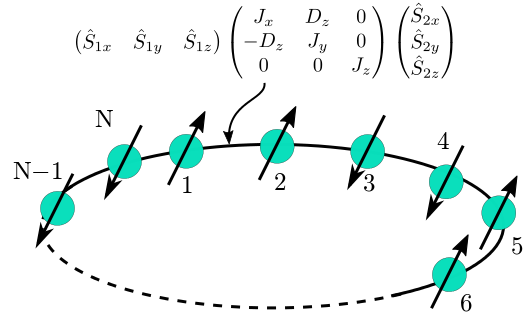
\includegraphics{spin.png}
\caption{1次元スピン系の模式図.}\label{shiftk_format_ja:spin}\end{figure}
\begin{gather}
\begin{split}\begin{align}
  {\hat H} = \sum_{i}
  \left(
  \begin{matrix}
    {\hat S}_{i x} & {\hat S}_{i y} & {\hat S}_{i z}
  \end{matrix}
  \right)
  \left(
  \begin{matrix}
    J_x & D_z & 0 \\
    -D_z & J_y & 0 \\
    0 & 0 & J_z
  \end{matrix}
  \right)
  \left(
  \begin{matrix}
    {\hat S}_{i+1 x} \ {\hat S}_{i+1 y} \ {\hat S}_{i+1 z}
  \end{matrix}
  \right)\end{align}\end{split}\notag
\end{gather}\begin{itemize}
\item {} 
\code{nsite}

\textbf{形式 :} 整数 (default: \code{4})

\textbf{説明 :} 1次元スピン模型のサイト数を指定します.

\item {} 
\code{Jx}

\textbf{形式 :} 実数 (default: \code{1.0})

\textbf{説明 :} Heisenberg模型の \(J_x\) を指定します.

\item {} 
\code{Jy}

\textbf{形式 :} 実数 (default: \code{1.0})

\textbf{説明 :} Heisenberg模型の \(J_y\) を指定します.

\item {} 
\code{Jz}

\textbf{形式 :} 実数 (default: \code{1.0})

\textbf{説明 :} Heisenberg模型の \(J_z\) を指定します.

\item {} 
\code{Dz}

\textbf{形式 :} 実数 (default: \code{0.0})

\textbf{説明 :}
Dzyaloshinskii-Moriya相互作用のパラメーター \(D_z\) を指定します.

\end{itemize}

\code{cg}
ネームリストでは(双)共役勾配法の反復に関するパラメーターを指定します.
\begin{itemize}
\item {} 
\code{MaxLoops}

\textbf{形式 :} 整数 (default: ハミルトニアンの次元)

\textbf{説明 :} 最大反復回数を指定します.

\item {} 
\code{Convfactor}

\textbf{形式 :} 整数 (default: \code{8})

\textbf{説明 :} 残差ベクトルの二乗ノルムを次元数で割ったものが,
\(10^{-{\tt Convfactor}}\) 未満となったら収束したとみなして計算を終了します.

\end{itemize}

\code{dyn} ネームリストではスペクトルの計算に関するパラメーターを指定します.
\begin{itemize}
\item {} 
\code{OmegaMin}

\textbf{形式 :} 複素数 (default: \code{invec} を指定しなかった場合には
(ハミルトニアンの最小固有値,
最大 \(\cdot\) 最小固有値の差 \(\times0.01\)),
それ以外の場合には \code{(0.0, 0.01)})

\textbf{説明 :} 振動数の始点を指定します.

\item {} 
\code{OmegaMax}

\textbf{形式 :} 複素数 (default: \code{invec} を指定しなかった場合には
(ハミルトニアンの最大固有値,
最大 \(\cdot\) 最小固有値の差 \(\times0.01\)),
それ以外の場合には \code{(1.0, 0.01)})

\textbf{説明 :} 振動数の終点を指定します.

\item {} 
\code{NOmega}

\textbf{形式 :} 整数 (default: \code{10})

\textbf{説明 :} 振動数の点数を指定します.

\item {} 
\code{outrestart}

\textbf{形式 :} 論理型 (default: \code{.FALSE.})

\textbf{説明 :}
リスタート用ファイルを出力するか( \code{.TRUE.})否か( \code{.FALSE.})を指定します.

\item {} 
\code{calctype}

\textbf{形式 :}
String型.  \code{"normal"}, \code{"recalc"}, \code{"restart"} のいずれか.
(default: \code{"normal"})

\textbf{説明 :}
\code{"normal"} が指定された場合にはKrylov部分空間法をはじめから行います.
\code{"recalc"} の場合には先行する計算で出力されたリスタート用ファイルを読み込み
先行する計算で行われたのと同じ反復回数まで計算します. 収束は保証されません.
\code{"restart"} では先行する計算で出力されたリスタート用ファイルを読み込み,
先行する計算で行われたのと同じ反復回数まで計算したのち,
収束するか最大反復回数( \code{MaxLoops})に達するまで計算を続けます.

\end{itemize}


\subsection{InHamファイル}
\label{shiftk_format_ja:inham}\label{shiftk_format_ja:ham}
MatrixMarket形式に準じ, 以下のフォーマットを採用しています.

InHamファイルの例

\begin{Verbatim}[commandchars=\\\{\}]
\PYGZpc{}\PYGZpc{}MatrixMarket matrix coordinate complex hermitian
16 16 20
1 1 1.000000 0.000000
3 2 0.500000 0.000000
5 3 0.500000 0.000000
6 4 0.500000 0.000000
6 6 \PYGZhy{}1.000000 0.000000
7 6 0.500000 0.000000
9 2 0.500000 0.000000
9 5 0.500000 0.000000
10 6 0.500000 0.000000
11 4 0.500000 0.000000
11 7 0.500000 0.000000
11 10 0.500000 0.000000
11 11 \PYGZhy{}1.000000 0.000000
12 8 0.500000 0.000000
13 6 0.500000 0.000000
13 11 0.500000 0.000000
14 12 0.500000 0.000000
15 8 0.500000 0.000000
15 14 0.500000 0.000000
16 16 1.000000 0.000000
\end{Verbatim}
\begin{description}
\item[{1行目:}] \leavevmode
任意の文字列(コメントなど)が入ります.

\item[{2行目:}] \leavevmode
行数, 列数, 非ゼロ要素の数が入ります.
非ゼロ要素数に関しては \textbf{行列の下三角部分のみ} の数を記入してください.

\item[{3行目以降:}] \leavevmode
行番号, 列番号, 要素の実部, 要素の虚部が入ります.
2行目で入れた, 非ゼロ要素数と同じ数(下三角部分のみ)記入してください.

\end{description}


\subsection{InVecファイル}
\label{shiftk_format_ja:invec}\label{shiftk_format_ja:vec}
励起ベクトルを入力するテキスト形式のファイルです.
ファイル名は入出力ファイル指定ファイルで指定します.
以下のようなフォーマットをしています.

\begin{Verbatim}[commandchars=\\\{\}]
8192
0.02 0.01
0.02 0.001
(continue...)
\end{Verbatim}
\begin{itemize}
\item {} 
1行目: {[} int01 {]}

\textbf{形式 :} int型

\textbf{説明 :} 計算対象のヒルベルト空間数を指定する整数.
ハミルトニアンの次元と一致している必要があります.

\item {} 
2行目-:
{[} double01 {]} {[} double02 {]}

\textbf{形式 :} double型

\textbf{説明 :} 励起ベクトルの値を表します.
{[} double01 {]} が実部, {[} double02 {]} が虚部を表します.

\end{itemize}


\subsection{リスタート用係数}
\label{shiftk_format_ja:id4}\label{shiftk_format_ja:recoeff}
リスタート用の係数を入力するテキスト形式のファイルです.
ファイル名は \code{TriDiagComp.dat} です.
以下のようなフォーマットをしています.

\begin{Verbatim}[commandchars=\\\{\}]
1000
1.0 0.0
0.1 0 0.01  0
0.2 0 0.021 0
(continue...)
2.1 \PYGZhy{}0.5
3.1 4.0
(continue...)
\end{Verbatim}
\begin{itemize}
\item {} 
1行目: {[} int01 {]}

\textbf{形式 :} int型

\textbf{説明 :}
\(\alpha, \beta\) の読み込み総数を表します. 前回計算時のイタレーション数に相当します.

\item {} 
2行目: {[} double01 {]} {[} double02 {]}

\textbf{形式 :} double型

\textbf{説明 :} シード振動数 \(z_{\rm seed}\) の値を表します.
{[} double01 {]} が \(z_{\rm seed}\) の実部,
{[} double02 {]} が \(z_{\rm seed}\) の虚部を表します.

\item {} 
3行目-2+ {[} int01 {]} 行目:
{[} double03 {]} {[} double04 {]} {[} double05 {]} {[} double06 {]}

\textbf{形式 :} double型

\textbf{説明 :} \(\alpha, \beta\) の値を表します.
{[} double03 {]} が \(\alpha\) の実部, {[} double04 {]} が \(\alpha\) の虚部,
{[} double05 {]} が \(\beta\) の実部, {[} double06 {]} が \(\beta\) の虚部を表します.

\item {} 
3+ {[} int01 {]} 行目-2 + 2 \(\times\) {[} int01 {]} 行目:
{[} double07 {]} {[} double08 {]}

\textbf{形式 :} double型

\textbf{説明 :} 各反復での残差ベクトルと励起ベクトルの内積を表します.
{[} double07 {]} が実部, {[} double08 {]} が虚部を表します.

\end{itemize}


\subsection{リスタート用ベクトル}
\label{shiftk_format_ja:id5}\label{shiftk_format_ja:revec}
リスタート用ベクトルを入力するテキスト形式のファイルです.
ファイル名は \code{ResVec.dat} です.
以下のようなフォーマットをしています.

\begin{Verbatim}[commandchars=\\\{\}]
8192
0.02 0.01
0.02 0.001
(continue...)
0.02 0.01
0.02 0.001
(continue... Only for BiCG)
\end{Verbatim}
\begin{itemize}
\item {} 
1行目: {[} int01 {]}

\textbf{形式 :} int型

\textbf{説明 :} 計算対象のヒルベルト空間数を指定する整数.

\item {} 
2行目-1+ {[} int01 {]} 行目:
{[} double01 {]} {[} double02 {]}

\textbf{形式 :} double型

\textbf{説明 :} 残差ベクトルの値を表します.
{[} double01 {]} が実部, {[} double02 {]} が虚部を表します.

\item {} 
3行目-1+ \(2\times[\) int01 {]} 行目:
{[} double03 {]} {[} double04 {]}

\textbf{形式 :} double型

\textbf{説明 :}
(ハミルトニアンが複素の場合のみ出力)影の残差ベクトルの値を表します.
{[} double03 {]} が実部, {[} double04 {]} が虚部を表します.

\end{itemize}


\section{出力ファイル}
\label{shiftk_format_ja:id6}

\subsection{リスタート用係数}
\label{shiftk_format_ja:id7}
Sec. {\hyperref[shiftk_format_ja:recoeff]{\emph{リスタート用係数}}} と同じ形式を取ります.


\subsection{リスタート用ベクトル}
\label{shiftk_format_ja:id8}
Sec. {\hyperref[shiftk_format_ja:revec]{\emph{リスタート用ベクトル}}} と同じ形式を取ります.


\subsection{動的グリーン関数ファイル}
\label{shiftk_format_ja:dynamicalg}\label{shiftk_format_ja:id9}
動的グリーン関数の計算結果を出力するテキスト形式のファイルです.
以下のようなフォーマットをしています.

\begin{Verbatim}[commandchars=\\\{\}]
\PYGZhy{}10 0.001 0.001 \PYGZhy{}0.0001
\PYGZhy{}9.8 0.001 0.0012 \PYGZhy{}0.0002
\PYGZhy{}9.6 0.001 0.0014 \PYGZhy{}0.0003
(continue...)
\end{Verbatim}
\begin{itemize}
\item {} 
1行目-:
{[} double01 {]} {[} double02 {]} {[} double03 {]} {[} double04 {]}
\begin{itemize}
\item {} 
{[} double01 {]}, {[} double02 {]}

\textbf{形式 :} double型

\textbf{説明 :} 周波数数の実部
{[} double01 {]} と虚部 {[} double02 {]} を表します.

\item {} 
{[} double03 {]}, {[} double04 {]}

\textbf{形式 :} double型

\textbf{説明 :} 動的グリーン関数の値を表します.
{[} double01 {]} が実部, {[} double02 {]} が虚部を表します.

\end{itemize}

\end{itemize}


\chapter{Contact}
\label{shiftk_contact_ja:contact}\label{shiftk_contact_ja::doc}
このミニアプリについてのご意見, ご質問,
バグ報告等ありましたら下記までお問い合わせください。

河村光晶

\begin{Verbatim}[commandchars=\\\{\}]
\PYG{n}{mkawamura\PYGZus{}at\PYGZus{}issp}\PYG{o}{.}\PYG{n}{u}\PYG{o}{\PYGZhy{}}\PYG{n}{tokyo}\PYG{o}{.}\PYG{n}{ac}\PYG{o}{.}\PYG{n}{jp}
\end{Verbatim}

\code{\_at\_} を \code{@} に変えてください.



\renewcommand{\indexname}{索引}
\printindex
\end{document}
